% !TeX root = RJwrapper.tex
\title{Reproducible Summary Tables with gtsummary}
\author{by Daniel D. Sjoberg, Karissa Whiting, Margie Hannum, Michael Curry}

\maketitle

\abstract{
An abstract of less than 150 words.
}

\section{Introduction}

\section{Data Summaries}

% adding table describing trial dataset
\captionsetup[table]{labelformat=empty,skip=1pt}
\begin{longtable}{llll}
\toprule
colname & label & class & values \\ 
\midrule
\texttt{trt} & Chemotherapy Treatment & character & \texttt{Drug A}, \texttt{Drug B} \\ 
\texttt{age} & Age & numeric & \texttt{6}, \texttt{9}, \texttt{10}, \texttt{17}, ... \\ 
\texttt{marker} & Marker Level (ng/mL) & numeric & \texttt{0.003}, \texttt{0.005}, \texttt{0.013}, \texttt{0.015}, ... \\ 
\texttt{stage} & T Stage & factor & \texttt{T1}, \texttt{T2}, \texttt{T3}, \texttt{T4} \\ 
\texttt{grade} & Grade & factor & \texttt{I}, \texttt{II}, \texttt{III} \\ 
\texttt{response} & Tumor Response & integer & \texttt{0}, \texttt{1} \\ 
\texttt{death} & Patient Died & integer & \texttt{0}, \texttt{1} \\ 
\texttt{ttdeath} & Months to Death/Censor & numeric & \texttt{3.53}, \texttt{5.33}, \texttt{6.32}, \texttt{7.27}, ... \\ 
\bottomrule\caption{\label{tab:caption}Table 1. Example data frame, \texttt{trial}}\\

\end{longtable}




\subsection{\texorpdfstring{\texttt{tbl\_summary()}}{tbl\_summary()}}

% code for basic tbl_summary()
\begin{example}
trial %>%
  select(age, grade, response, trt) %>%
  tbl_summary(by = trt)
\end{example}
\begin{figure}[h!]
  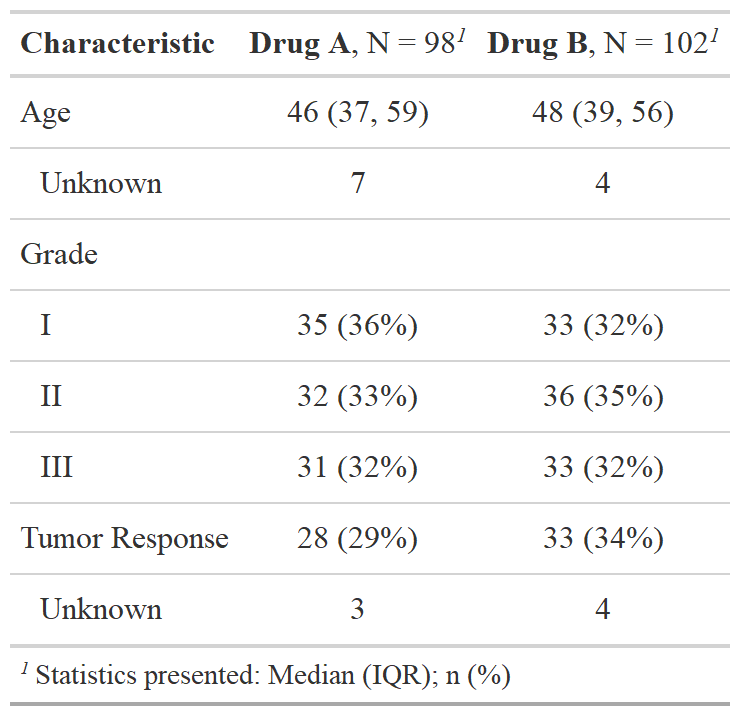
\includegraphics[height=5cm]{summary_basic.png}
  \centering
\end{figure}


% code for tbl_summary() with arguments
\captionsetup[table]{labelformat=empty,skip=1pt}
\begin{longtable}{ll}
\toprule
Argument & Description \\ 
\midrule
\texttt{label=} & specify the variable labels printed in table \\ 
\texttt{type=} & specify the variable type (e.g., continuous, categorical, etc.) \\ 
\texttt{statistic=} & change the summary statistics presented \\ 
\texttt{digits=} & number of digits the summary statistics will be rounded to \\ 
\texttt{missing=} & whether to display a row with the number of missing observations \\ 
\texttt{missing\_text=} & text label for the missing number row \\ 
\texttt{sort=} & change the sorting of categorical levels by frequency \\ 
\texttt{percent=} & print column, row, or cell percentages \\ 
\texttt{include=} & list of variables to include in summary table \\ 
\caption{\label{tab:}\texttt{tbl\_summary()} function arguments}\\
\bottomrule
\end{longtable}


\begin{example}
trial %>%
  select(age, grade, response, trt) %>%
  tbl_summary(
    by = trt,
    type = all_continuous() ~ "continuous2",
    label = age ~ "Patient Age",
    statistic = list(all_continuous() ~ c("{N_nonmiss}", 
                                          "{mean} ({sd})", 
                                          "{median} ({p25}, {p75})", 
                                          "{min}, {max}"),
                     all_categorical() ~ "{n} / {N} ({p}%)"),
    digits = all_categorical() ~ c(0, 0, 1),
    missing = "no"
  )
\end{example}
\begin{figure}[h!]
  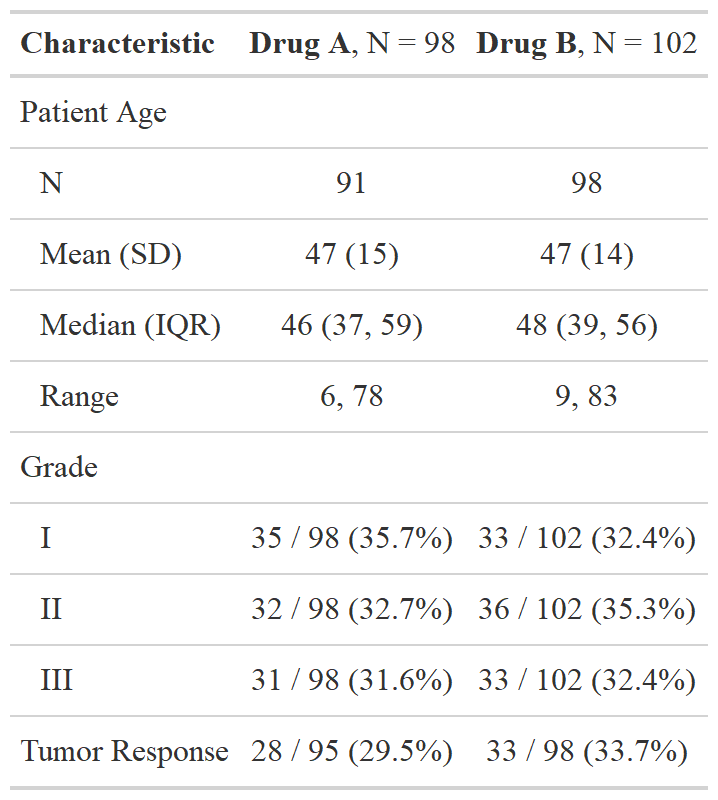
\includegraphics[height=5cm]{summary_plus.png}
  \centering
\end{figure}

% code for tbl_summary() with arguments
\captionsetup[table]{labelformat=empty,skip=1pt}
\begin{longtable}{ll}
\toprule
Function & Description \\ 
\midrule
\texttt{add\_p()} & add \emph{p}-values to the output comparing values across groups \\ 
\texttt{add\_overall()} & add a column with overall summary statistics \\ 
\texttt{add\_n()} & add a column with N (or N missing) for each variable \\ 
\texttt{add\_difference()} & add column for difference between two group, confidence interval, and \emph{p}-value \\ 
\texttt{add\_stat\_label()} & add label for the summary statistics shown in each row \\ 
\texttt{add\_stat()} & generic function to add a column with user-defined values \\ 
\texttt{add\_q()} & add a column of \emph{q}-values to control for multiple comparisons \\ 
\bottomrule\caption{\label{tab:caption}Table 3. \texttt{tbl\_summary()} functions to add information}\\

\end{longtable}


\begin{example}
trial %>%
  select(age, grade, response, trt) %>%
  tbl_summary(by = trt, missing = "no") %>%
  add_p(test = all_continuous() ~ "t.test",
        pvalue_fun = ~style_pvalue(., digits = 2)) %>%
  add_n()
\end{example}
\begin{figure}[h!]
  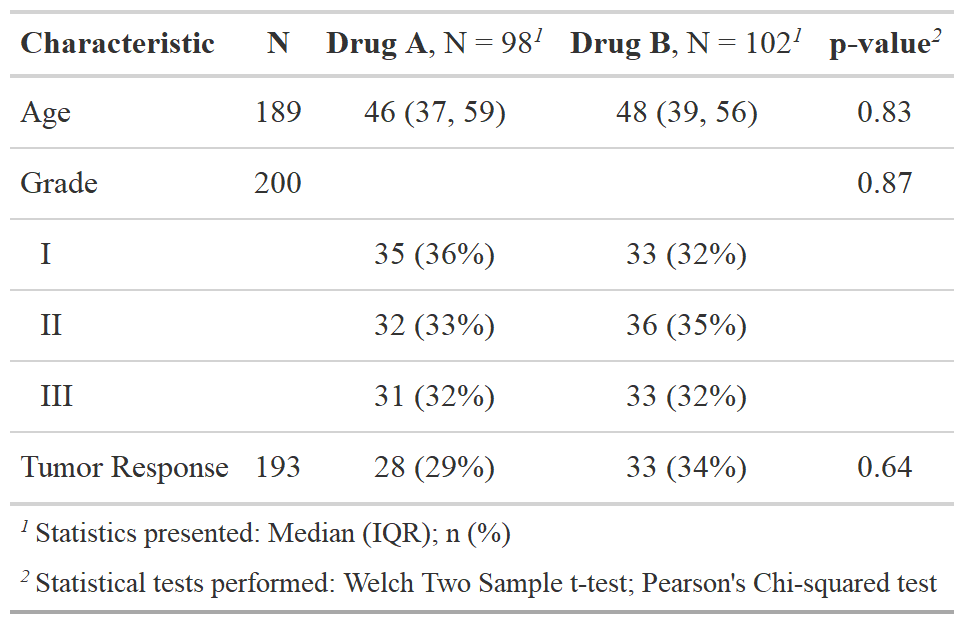
\includegraphics[height=5cm]{summary_plus_plus.png}
  \centering
\end{figure}

\subsection{\texorpdfstring{\texttt{tbl\_svysummary()}}{tbl\_svysummary()}}

\subsection{\texorpdfstring{\texttt{tbl\_cross()}}{tbl\_cross()}}

\subsection{\texorpdfstring{\texttt{tbl\_survfit()}}{tbl\_survfit()}}

\subsection{Customization}

\section{Model Summaries}

\subsection{\texorpdfstring{\texttt{tbl\_regression()}}{tbl\_regression()}}

\hypertarget{tbl_uvregression}{%
\subsection{\texorpdfstring{\texttt{tbl\_uvregression()}}{tbl\_uvregression()}}\label{tbl_uvregression}}

\hypertarget{in-line-reporting}{%
\section{In-line Reporting}\label{in-line-reporting}}

\hypertarget{merging-and-stacking}{%
\section{Merging and Stacking}\label{merging-and-stacking}}

\hypertarget{themes}{%
\section{Themes}\label{themes}}

\hypertarget{print-engines}{%
\section{Print Engines}\label{print-engines}}

\bibliography{RJreferences}

\address{Author One\\
  Affiliation\\
  Address\\
  Country\\
  (ORCiD if desired)\\
  \email{author1@work}}

\address{Author Two\\
  Affiliation\\
  Address\\
  Country\\
  (ORCiD if desired)\\
  \email{author2@work}}

\address{Author Three\\
  Affiliation\\
  Address\\
  Country\\
  (ORCiD if desired)\\
  \email{author3@work}}
